\section{Resultados}

\subsection{Modelo de fuente \texorpdfstring{$S_1$}{S1}}

A continuación se dispone el análisis de los resultados obtenidos modelando las redes como fuentes de información con memoria nula.

\subsubsection{Red corporativa}

Los siguientes graficos muestran para cada red la información para cada uno de sus símbolos capturados, las probabilidades de que estos sean registrados, la entropía registrada y la entropía máxima.

\begin{figure}[H]
	\begin{minipage}{0.49\textwidth}
		\centering
		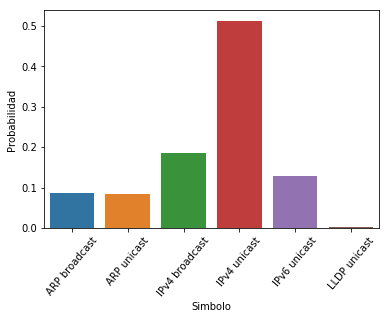
\includegraphics[width=\linewidth]{imagenes/despegar_barras_prob}
		\caption{Red corporativa - Probabilidad}
		\label{despe_barras_prob}
	\end{minipage}
	\begin{minipage}{0.49\textwidth}
		\centering
		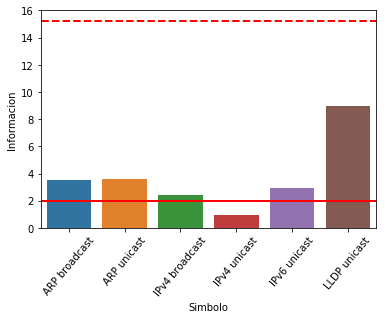
\includegraphics[width=\linewidth]{imagenes/despegar_barras_info}
		\caption{Red corporativa - Información}
		\label{despe_barras_info}
	\end{minipage}
\end{figure}

Sobre esta red observamos un trafico medianamente distriubido de los símbolos obtenidos. La mitad de ellos son \texttt{IPV4 UNICAST}, casi un 20 \% de \texttt{IPV4 BROADCAST} y entre 12\% y 8\% el resto. Puede verse una gran cantidad de informacion proveniente del símbolo \texttt{LLDP UNICAST}. Este protocolo es conocido cómo \textit{Link Layer Discovery Protocol}. La prescencia de este tipo de paquete se explica con que se usa como un componente en aplicaciones de administración y monitoreo de red, lo cual es común en redes corporativas. La baja frecuencia de este tipo de paquete repercute en que la información del símbolo sea muy alta.

Con el fin de realizar un análisis más exhaustivo, resulta útil estudiar los porcentajes relativos de aparición de los distintos símbolos de la fuente S1 para cada red.

\begin{figure}[H]
	\begin{minipage}{0.49\textwidth}
		\centering
		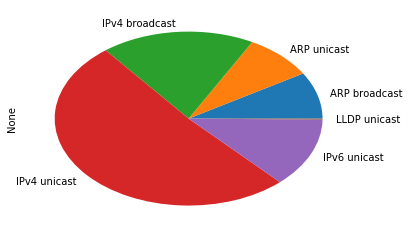
\includegraphics[width=\linewidth]{imagenes/despegar_torta_simbolos}
		\caption{Red corporativa - Símbolos}
		\label{despe_torta_simb}
	\end{minipage}
	\begin{minipage}{0.49\textwidth}
		\centering
		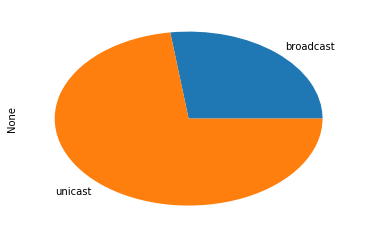
\includegraphics[width=\linewidth]{imagenes/despegar_torta_tipos}
		\caption{Red corporativa - Tipos}
		\label{despe_torta_tipos}
	\end{minipage}
\end{figure}

En este caso, existe una desproporción entre paquetes broadcast y unicast. Sin embargo, la proporción de paquetes broadcast y además la cantidad de paquetes ARP parece indicar que existe bastante interacción entre los nodos dentro de la red.

\subsubsection{Red pública (McDonald's)}

\begin{figure}[H]
	\begin{minipage}{0.49\textwidth}
		\centering
		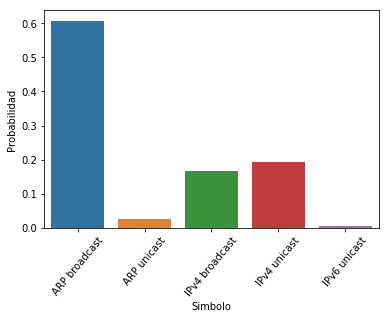
\includegraphics[width=\linewidth]{imagenes/mac_barras_prob}
		\caption{Red pública(McDonald's) - Probabilidad}
		\label{mac_barras_prob}		
	\end{minipage}
	\begin{minipage}{0.49\textwidth}
		\centering
		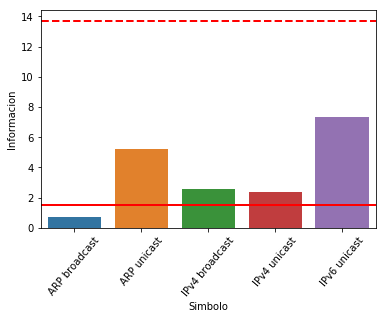
\includegraphics[width=\linewidth]{imagenes/mac_barras_info}
		\caption{Red pública(McDonald's) - Información}
		\label{mac_barras_info}		
	\end{minipage}
\end{figure}

La principal motivación para estudiar la red de McDonald's fue poder observar un medio con mucha entrada y salida de dispositivos, el hecho de que se tratara de una red inalámbrica permitió además contrastar las diferencias frente a la primer captura sobre una red cableada. Se nota la gran cantidad de paquetes \texttt{ARP BROADCAST}, son el 60\% de los capturados. Nuestra hipótesis es que la continua fluctuación de hosts en esta red provoca que se disparen muchos paquetes de control para mantener actualizado el estado de la misma.

\begin{figure}[H]
	\begin{minipage}{0.49\textwidth}
		\centering
		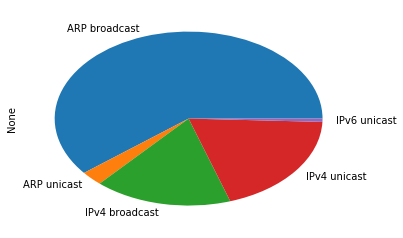
\includegraphics[width=\linewidth]{imagenes/mac_torta_simbolos}
		\caption{Red pública(McDonald's) - Símbolos}
		\label{mac_torta_simb}
	\end{minipage}
	\begin{minipage}{0.49\textwidth}
		\centering
		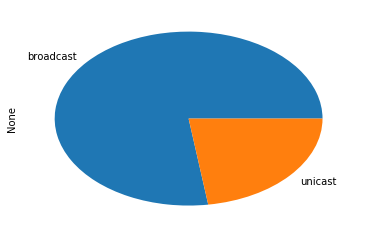
\includegraphics[width=\linewidth]{imagenes/mac_torta_tipos}
		\caption{Red pública(McDonald's) - Tipos}
		\label{mac_torta_tipos}
	\end{minipage}
\end{figure}

En la captura realizada sobre la red pública podemos ver que la cantidad de paquetes destinados al control de la red es considerablemente mayor con respecto a las red corporativa y la doméstica. Una posible hipótesis a este resultado es el hecho de que al ser una red de muchos hosts donde varios de ellos se comunican entre sí es necesario para estos mantener actualizada la información sobre la red. Es interesante observar la cantidad de paquetes tipo \texttt{IPV4 Broadcast}, este tipo de paquete es mayormente utilizado por protocolos de capas superiores, como NetBT, para tener más una mayor información sobre la red, ya que en un ambiente corporativo es muy necesario para detectar errores rápidamente.

\subsubsection{Red doméstica}

\begin{figure}[H]
	\begin{minipage}{0.49\textwidth}
		\centering
		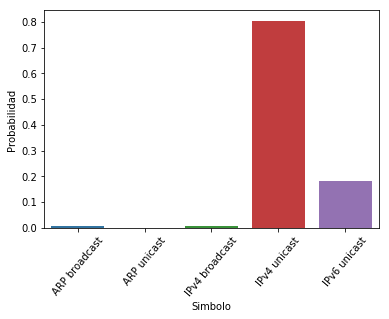
\includegraphics[width=\linewidth]{imagenes/manu_casa_barras_prob}
		\caption{Red doméstica - Probabilidad}
		\label{casa_barras_prob}
	\end{minipage}
	\begin{minipage}{0.49\textwidth}
		\centering
		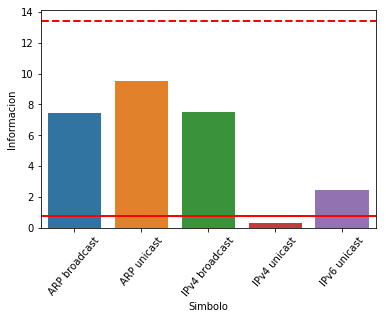
\includegraphics[width=\linewidth]{imagenes/manu_casa_barras_info}
		\caption{Red doméstica - Información}
		\label{casa_barras_info}
	\end{minipage}
\end{figure}

Para el grafico de la red doméstica podemos observar un predominancia en los paquetes \texttt{IPV4 UNICAST}, conformando mas de un 80\% de los paquetes que transitan por la red, seguido por un 18\% de paquetes \texttt{IPV6 UNICAST}. La entropía es de 0.797. Este número resulta mucho mas baja que las demás, y creemos que se debe justamente a que la gran mayoría de los paquetes es \texttt{UNICAST}, y esto provoca que el tráfico de la red sea fácil de predecir.

\begin{figure}[H]
	\begin{minipage}{0.49\textwidth}
		\centering
		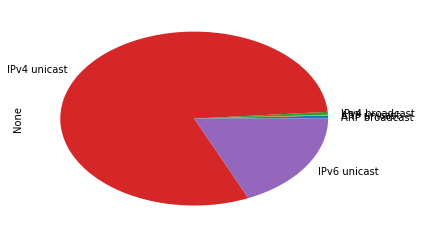
\includegraphics[width=\linewidth]{imagenes/manu_casa_torta_simbolos}
		\caption{Red doméstica - Símbolos}
		\label{casa_torta_simb}
	\end{minipage}
	\begin{minipage}{0.49\textwidth}
		\centering
		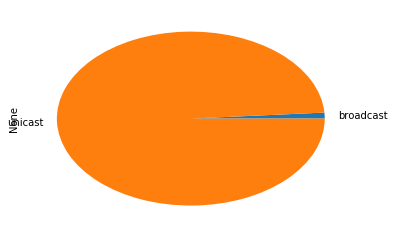
\includegraphics[width=\linewidth]{imagenes/manu_casa_torta_tipos}
		\caption{Red doméstica - Tipos}
		\label{casa_torta_tipos}
	\end{minipage}
\end{figure}

Como puede observarse en los gráficos, los resultados obtenidos para la fuente $S_1$ muestran que los paquetes de tipo broadcast son casi inexistentes. Este fenómeno se puede explicar, por el siguiente motivo: los paquetes de tipo broadcast suelen corresponder con protocolos de control, como ARP, y dado que las comunicaciones en general se dan exclusivamente entre el default gateway y los demás nodos, los protocolos de control no son requeridos.


\subsection{Modelo de fuente \texorpdfstring{$S_2$}{S2}}

Este modelo contiene símbolos de la forma $< tipo de paquete ARP, IP destino >$

Cabe destacar los cambios en la cantidad de símbolos con el modelo anterior. Este hace una distinción por cada host distinto dentro de las capturas, y al tener capturas en las que hay muchos dispositivos en juego, la cantidad de símbolos distintos aumenta linealmente con ellos.

Despegar S2 BARPLOT

Podemos observar que si bien hay más paquetes de tipo \texttt{WHO-HAS}, los paquete \texttt{IS-AT} no son pocos, casi el 25\% de los paquetes capturados, esto nos habla de una gran interacción entre los dispositivos pertenecientes a la red. También se puede apreciar que hay símbolos que aportan menos información que los demás. Puntualmente hay 6 símbolos de tipo \texttt{WHO-HAS} por debajo de la entropía, estos nodos distinguidos posiblemente sean las ips referidas a gateways o a servidores que deben ser recurridos frecuentemente por distintos usuarios.


